\section{Study Design and Evidence Boundary}
\label{sec:identity}
\subsection{The source performance protocol}
The source workflow, version 4.1, was intended to evaluate wind performance in stages. Its initial stage, B0, used predictor information only. It fixed station roles, satellite files, time blocks, predictor extracts, opportunity counts, processing states, transfer records, and later evaluation rules before any recorded request for National Data Buoy Center (NDBC) wind outcomes. A capacity gate, denoted G0-v4.1, controlled entry to B1. Only a pass could authorize access to outcomes at the four development stations. Outcomes at the eight evaluation stations would remain sealed until a later evaluation stage.

The gate required at least 400 unique evaluation opportunities and at least eight opportunities in every evaluation station--block cell. If the 96 primary files did not meet both requirements, the next complete eight-file alternate round could be activated. Four rounds were permitted. The protocol prohibited selecting individual files from a round, substituting stations, relaxing thresholds, or inspecting reference winds to decide how to repair the design.

All four rounds were exhausted without meeting the rule. The workflow recorded G0-v4.1 as failed and stopped with \texttt{FAIL\_EXHAUSTED}; B1 remained closed. Consequently, no wind model fitting, performance comparison, calibration analysis, or evaluation score was produced. The planned performance hypotheses remained untested.

\subsection{The subsequent integrity audit}
Version 5 was a separate audit defined after the capacity failure. It inherited the selected files, station roles, blocks, thresholds, processing states, and opportunity keys. Its purpose was to reconstruct the recorded decision without changing those inputs or reading wind outcomes.

The audit gate, G0-v5, tests consistency of that reconstruction. It compares input hashes, identifiers, counts, keys, processing-state distributions, transfer totals, raw-file disposition, predictor-file properties, gate states, and outcome-read counters with the preserved record. A pass means that the replay agrees with the source evidence; it does not mean that the benchmark has become ready for performance evaluation. Figure~\ref{fig:workflow} summarizes these two decisions.

\begin{figure*}[!t]
\centering
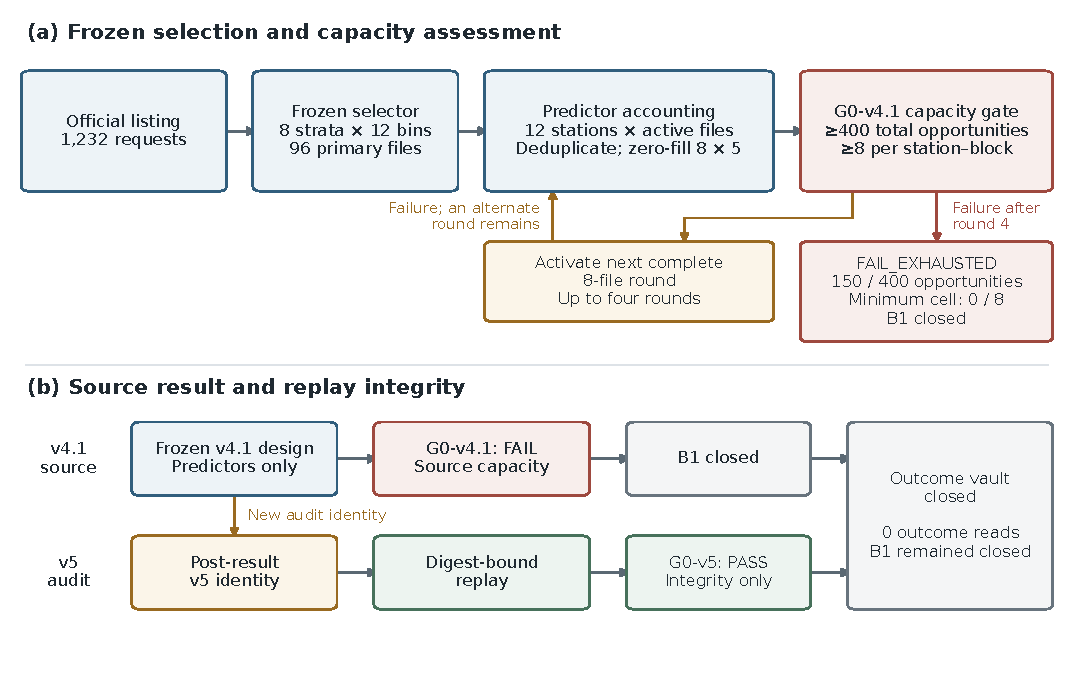
\includegraphics[width=\textwidth]{figures/figure1.pdf}
\caption{Readiness assessment and subsequent replay. The source workflow selects and processes files without opening buoy-wind outcomes, counts unique station--observation opportunities, and activates complete alternate rounds when needed. Failure after the final round stops performance evaluation. The later integrity audit checks the preserved failure record; its pass does not reverse the source decision.}
\label{fig:workflow}
\end{figure*}

The evidence boundary is the original repository record. Its counters report zero NDBC outcome reads, and the replay found no outcome paths or fields among its allowed inputs. This is an internal consistency claim, not a demonstration of external execution isolation. Because the audit was formulated after the capacity result was known, all findings in this paper remain exploratory.
